\chapter{Background}
\label{chapter2}

This project aims to improve the efficiency of real-time rendering of 3D fractals. This chapter will focus on background theory for fractals, signed distance functions and sphere tracing.

\section{2D Fractals - The Mandelbrot Set}

\begin{figure}[ht]
	\centering
	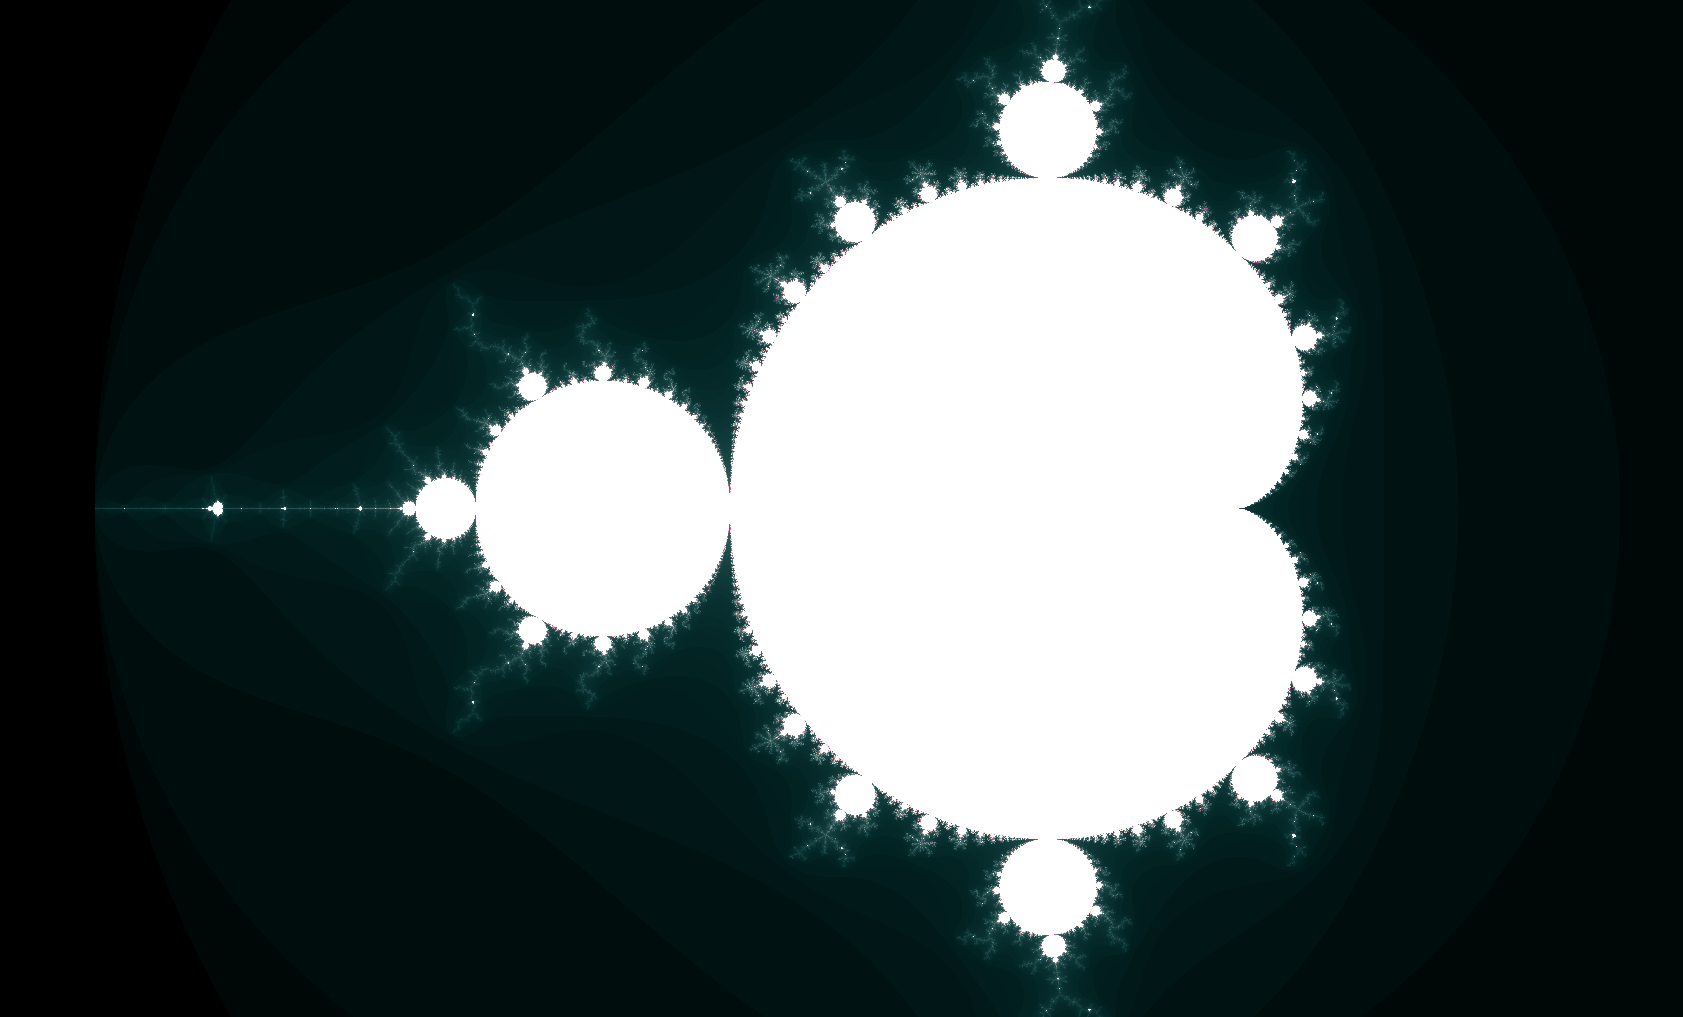
\includegraphics[width=0.65\linewidth, frame]{Images/Mandelbrot-2D-Full.png}
	\caption{The Mandelbrot set. The white points in the centre are inside the set.}
	\label{figure:mandelbrot-2d-full}
\end{figure}

The Mandelbrot set is the set of two-dimensional points that satisfy a certain constraint on the following complex quadratic equation:

\begin{equation} \label{equation:mandelbrot-2d}
	Z = {Z^2} + C
\end{equation}

where Z and C are complex numbers. The constraint on the points is that their orbit must be bounded. The value of Z is initialized to 0 and equation \ref{equation:mandelbrot-2d} is iterated over, each new value of Z being placed back in to the equation in the next iteration. If the length of the point Z does not exceed a threshold, then the point (represented by C) is in the Mandelbrot set \cite{devaney1999mandelbrot}.\newline

Figure \ref{figure:mandelbrot-2d-full} shows a generated Mandelbrot set. The real part of the point C is represented by the x-axis, and the imaginary part by the y-axis. Equation \ref{equation:mandelbrot-2d} is iterated over a maximum of five hundred times, and the threshold value is two. The pixels are coloured according to how many iterations are achieved before the length of Z exceeds the threshold.

\newpage

\begin{figure} [ht]
	\centering
	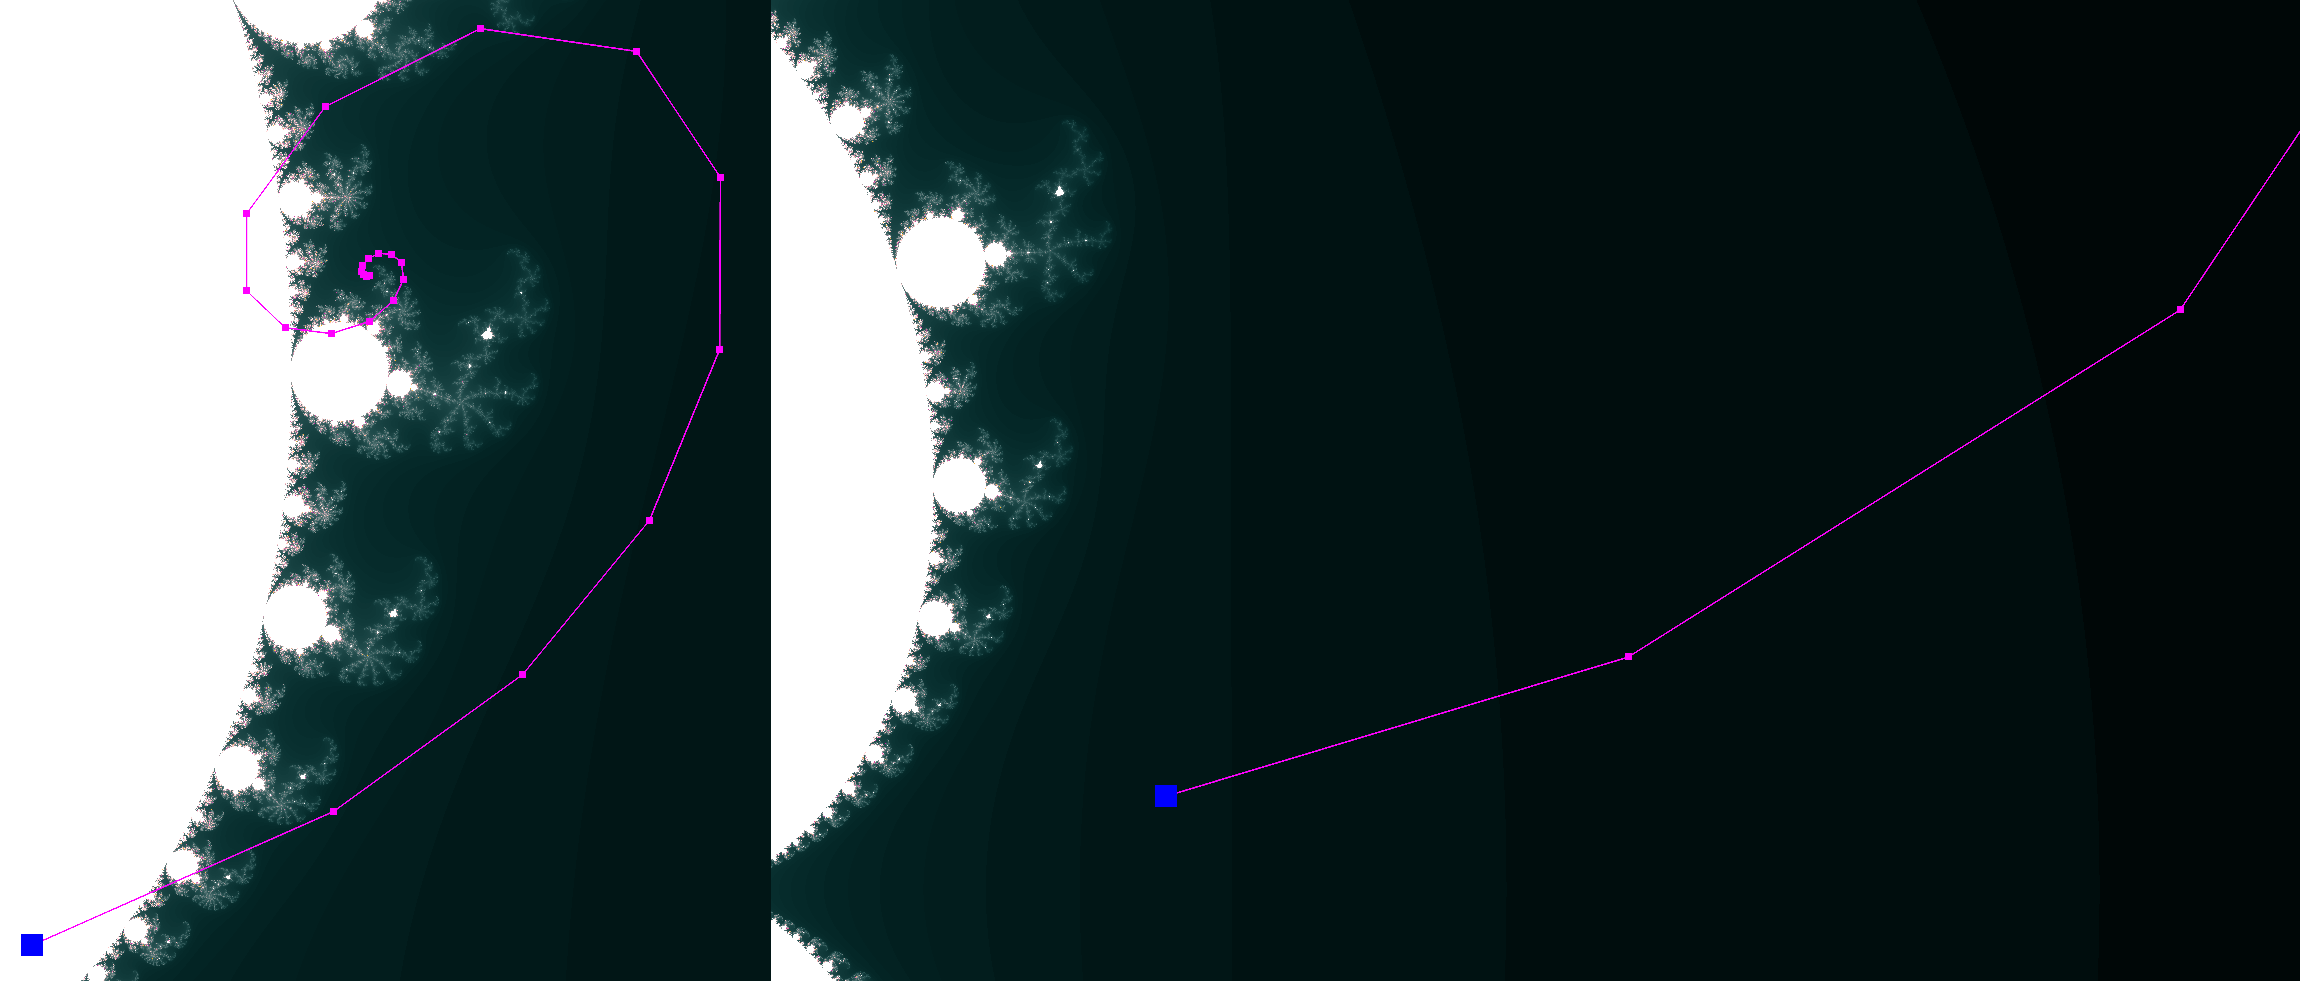
\includegraphics[width=\linewidth, frame]{Images/Mandelbrot-2D-Iterations.png}
	\caption{Visualization of the first twenty five iterations of equation \ref{equation:mandelbrot-2d} on the initial points [0.3, 0.05] (left) and [0.5, 0.04] (right). The initial points are shown in blue.}
	\label{figure:mandelbrot-2d-iterations}
\end{figure}

\begin{figure} [ht]
	\centering
	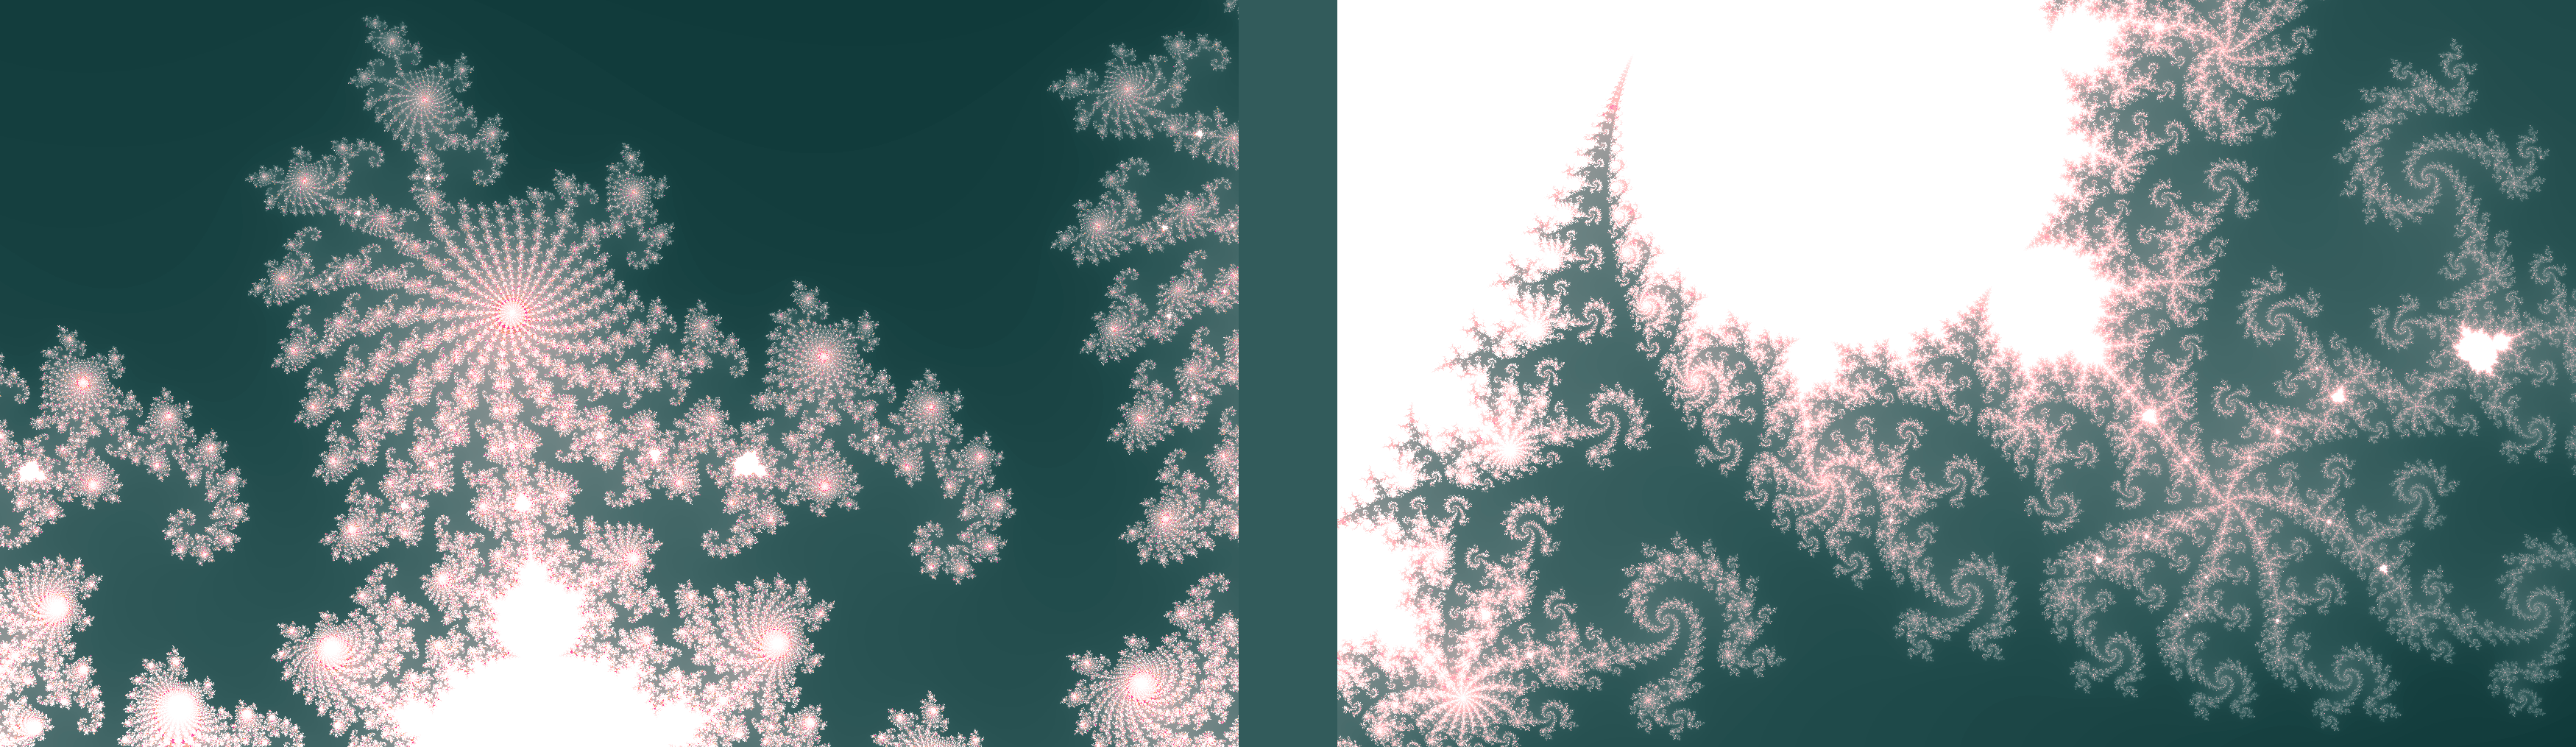
\includegraphics[width=\linewidth, frame]{Images/Mandelbrot-2D-Zoom.png}
	\caption{Two different views of the Mandelbrot set, zoomed in.}
	\label{figure:mandelbrot-2d-zoom}
\end{figure}

Figure \ref{figure:mandelbrot-2d-iterations} illustrates the first twenty five iterations on two different points. For the first point, the iterations converge in a spiral shape and the length of Z never exceeds the threshold of two, therefore the point is in the Mandelbrot set and is coloured white. For the second point, the iterations diverge and exceed the threshold of two within a few iterations, so this point is not in the Mandelbrot set and is coloured dark.\newline

Figure \ref{figure:mandelbrot-2d-zoom} shows two zoomed-in views at the edge of the original shape. New patterns can be seen, as well as repeated ones, and even new instances of the original shape. This is because the Mandelbrot set has infinite detail, so if one decreases the range of the axes, new patterns will emerge \cite{ashlock2006evolutionary}.\newline

This project makes use of three-dimensional fractal rendering, so the next section will look at the challenge of bringing this infinite level of detail to three dimensions.

\newpage

\section{3D Fractals - The Mandelbulb}

\begin{figure} [ht]
	\centering
	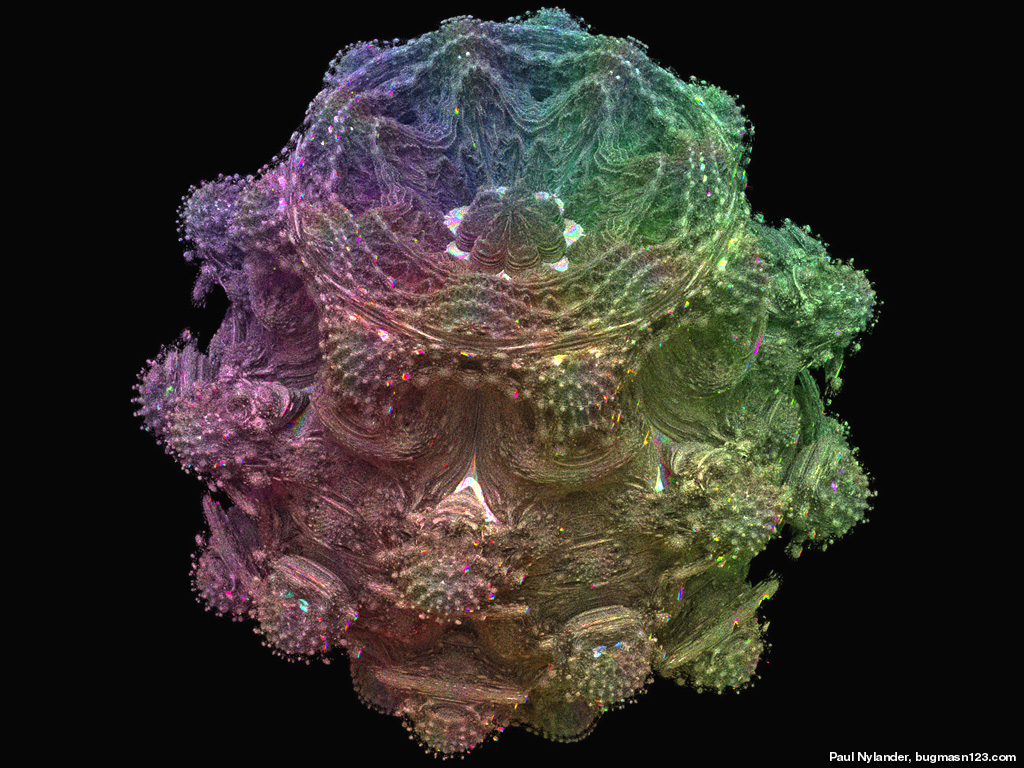
\includegraphics[width=0.5\linewidth, frame]{Images/Mandelbulb-First-Look.jpg}
	\caption{First look at the Mandelbulb, from Paul Nylander's website \cite{nylander-mandelbulb-image}.}
	\label{figure:mandelbulb-first-look}
\end{figure}

Since the Mandelbrot set is in two dimensions, and since complex numbers have only two components (real and imaginary), obtaining a true three-dimensional Mandelbrot set is a challenging task, and a mathematically rigorous three-dimensional Mandelbrot has not yet been found \cite{aron2009mandelbulb}.\newline

One attempt that seems to have come close was originated by Rudy Rucker in 1987. Rucker thought that expressing the three-dimensional points in spherical coordinates would allow the manipulation of the points in a similar way to the complex-number operations performed on the points in the two-dimensional Mandelbrot set \cite{rucker2009search}.\newline

Rucker did not have the computational power to accomplish a rendering of this idea, so it was put aside for twenty years, until Daniel White independently published a formula in 2007, which took the approach proposed by Rucker. White decided to approach the problem by considering the geometrical consequences of multiplying numbers in the complex plane, which amounts to rotating them \cite{aron2009mandelbulb}.\newline

White's formula produced images that looked promising, but they didn't have the level of detail that was expected from a true three-dimensional equivalent of the Mandelbrot set. A mathematician, Paul Nylander, raised White's formula to a higher power (eight), which would be equivalent to increasing the number of rotations of the point. The resulting image is shown in figure \ref{figure:mandelbulb-first-look}. The shape maintains excellent detail, even at high levels of magnification \cite {aron2009mandelbulb}.

\newpage

The new shape, known as the Mandelbulb, has roughly the same formula as the Mandelbrot set (equation \ref{equation:mandelbrot-2d}):

\begin{equation} \label{equation:mandelbulb}
	Z = {Z^k} + C
\end{equation}

where Z is raised to an arbitrary power like so:

\begin{equation} \label{equation:mandelbulb-power}
	{Z^k} = {r^k}(sin[k\theta]cos[k\phi], sin[k\theta]sin[k\phi], cos[k\theta]).
\end{equation}

The variable r is the norm of Z (|Z|), $\theta$ is equal to arctan($Z_y$/$Z_x$) and $\phi$ is equal to |($Z_x$, $Z_y$)|/$Z_z$. The spherical coordinates of the point Z/|Z| are represented by $\theta$ and $\phi$. Equations \ref{equation:mandelbulb} and \ref{equation:mandelbulb-power} are sourced from Chapter 33 of the book Ray Tracing Gems II \cite{marrs2021ray}.\newline

Papers:
\begin{itemize}
	\item The mandelbulb: first ‘true’3D image of famous fractal \cite{aron2009mandelbulb}.
	\item In Search of a Beautiful 3D Mandelbrot Set \cite{rucker2009search}.
	\item .
	\item A glimpse of the Mandelbulb with memory \cite{alonso2016glimpse}.
	\item On the Algebraic Foundation of the Mandelbulb \cite{boily2022algebraic}.
\end{itemize}

\section{Signed Distance Functions and Sphere Tracing}

Papers:
\begin{itemize}
	\item Ray Tracing Gems II \cite{marrs2021ray}.
\end{itemize}

- Briefly introduce ray tracing with triangle geometry.

- Signed distance function is an estimate of how close the point is to the surface of the fractal.

-  If it's negative, the point is inside the surface.

- Demonstrate derivation from Mandelbulb equation.

- Distance estimators can be used for raymarching - known as sphere tracing.

- Diagram of sphere tracing.

\section{Signed Distance Fields}

Papers:
\begin{itemize}
	\item Signed distance fields: A natural representation for both mapping and planning \cite{oleynikova2016signed}.
\end{itemize}

- Stored values from signed distance function, stored as 2D texture or 3D grid.

- Saves having to recompute SDF all the time.

- Fractal scenes with high view distance could benefit from some pre-calculated values to give them a head start - show room of pillars and remark on frame rate (no SDF).

- Remark on memory costs.

- Briefly talk about storage methods - octrees.

- Talk about 2D methods - particularly used for fonts.